\begin{frame}
    \begin{columns}
    
    \column[T]{0.58\textwidth}
    \begin{figure}
        \centering
            \begin{tikzpicture}
                \node (image) [anchor=south west, inner sep=0pt]  at (0,0) {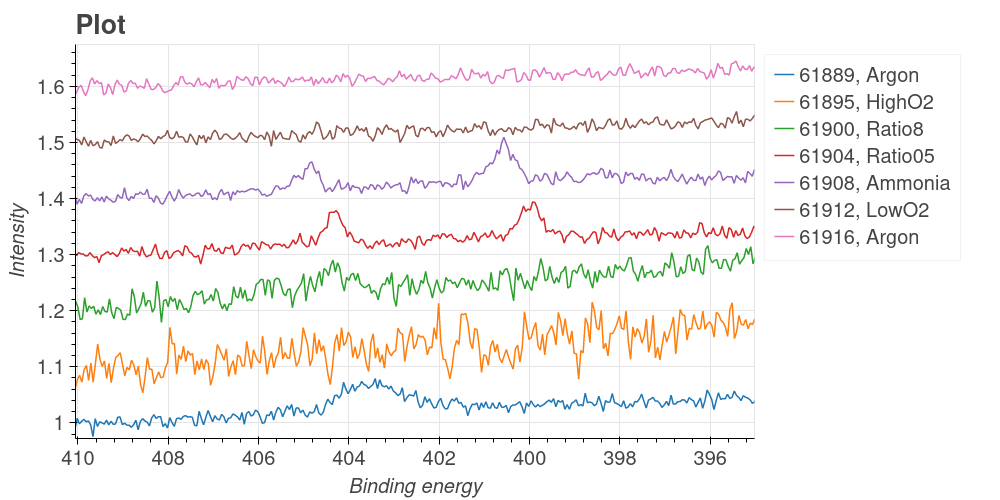
\includegraphics[width=0.8\textwidth, trim={0 0 8.3cm 1.4cm}, clip]{Figures/xps_data/N1sPt100.png}};

                \node (image) [anchor=south west, inner sep=0pt]  at (0,3.9) {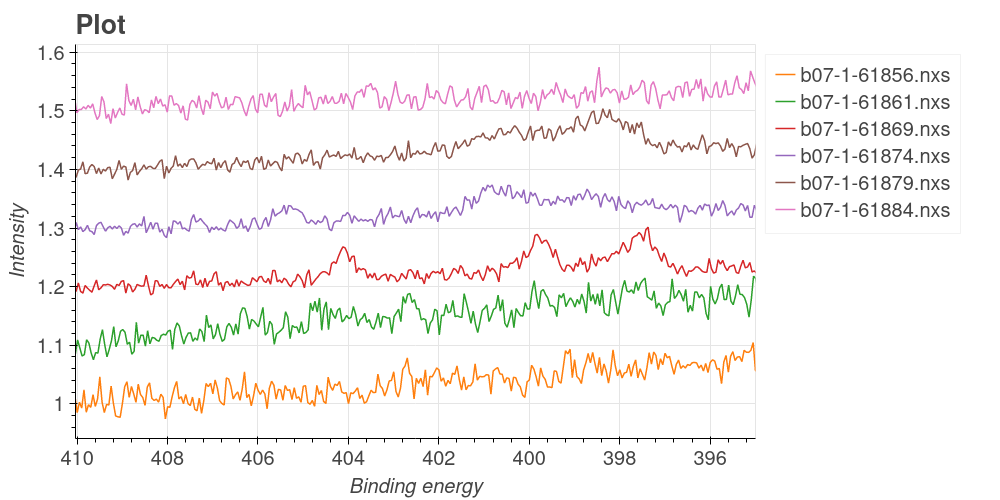
\includegraphics[width=0.8\textwidth, trim={0 0 8.3cm 1.4cm}, clip]{Figures/xps_data/N1sPt111.png}};

                \begin{scope}[x={(image.south east)}, y={(image.north west)}]
                    \node [fill=white, rounded corners=2pt, inner sep=1pt] at (0.1, 0.97) {\scriptsize Pt [100]};
                    \node [fill=white, rounded corners=2pt, inner sep=1pt] at (0.1, 0.45) {\scriptsize Pt [111]};
                \end{scope}
                
            \end{tikzpicture}
        \caption{N1s edge for Pt [100] (above) and Pt [111] (below)}
        \label{fig:N1s}
    \end{figure}
    
    \column[T]{0.4\textwidth}
    \begin{table}
        \centering
        \begin{tabular}{ |l|l|l| }
            \hline
            Argon & \ammonia & \dioxygen \\
            \hline
            \rowcolor{lightblue}
            10 & 0 & 0 \\
            \rowcolor{lightorange}
            0 & 0 & 8.8 \\
            \rowcolor{lightgreen}
            0 & 1.1 & 8.8 \\
            \rowcolor{lightred}
            0 & 1.1 & 0.55 \\
            \rowcolor{lightviolet}
            0 & 1.1 & 0 \\
            \rowcolor{lightbrown}
            10 & 0 & 0 \\
            \rowcolor{lightpink}
            0 & 0 & 0.55 \\
            \hline
        \end{tabular}
        \caption{Partial pressures in reactor (mbar), in experimental order.}
    \end{table}

    \begin{itemize}
        \item Peaks can only be clearly seen when the total pressure in below 2 mBar.
        \item One extra peak for Pt [100] in reaction conditions with more \ammonia than \dioxygen.
        \item The same peak is still here under pure Argon which would indicate a strongly adsorbed molecule.
    \end{itemize}

    \end{columns}
    
\end{frame}